\documentclass[11pt,letterpaper]{article}
\usepackage[applemac]{inputenc}
\usepackage{graphicx} 
\usepackage{html}
\usepackage{rotating}
\usepackage{palatino}
\author{David Reitter and Kevin Walzer}
\title{Aquamacs User Help}
\begin{document}
\maketitle

\tableofcontents
\pagebreak



\section{Aquamacs Emacs: a User-friendly Emacs Distribution}

Aquamacs is an freely-available Aqua-native build of the powerful Emacs text editor (\url{http://www.gnu.org/software/emacs/emacs.html}). By ``Aqua-native,'' we mean more than just the fact that this version of Emacs runs as a standard OS X application. Aquamacs features extensive customization that enables it to conform better with Apple's standard Human Interface Guidelines (HIG) than standard versions of the editor do. 

Emacs is a text editor of legendary power and configurability, but it
also has an enormously complex interface that, while consistent across
platforms, is usually at odds with the specific interface conventions
of the particular platform on which it is being used. The original GNU
version of Emacs for the Mac, called Carbon Emacs, is no different. 

Aquamacs Emacs implements the standard OS X keyboard
shortcuts and other interface conventions, integrating Emacs into the
Aqua environment to a far greater degree than other versions of
Emacs. This allows Mac users who might be unfamiliar with Emacs'
complex standard interface to harness its amazing editing power in a
familiar way. 

\begin{figure}
\centering
{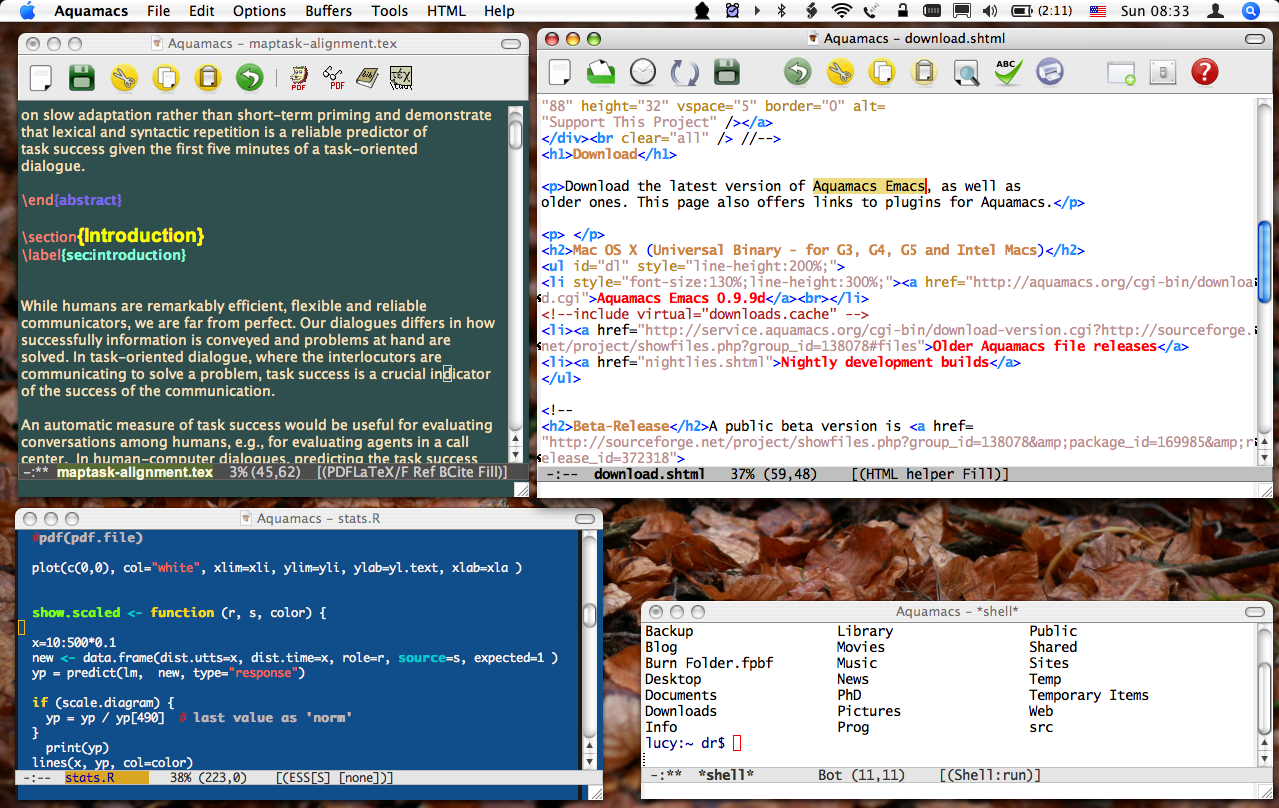
\includegraphics[width=5in]{aquamacs-screenshot.png}}
\caption{Aquamacs combines the legendary power of Emacs with
  user-friendly customizations to provide a more Aqua-specific user experience.}
\label{aquamacs-screenshot.jpg}
\end{figure}

You can always download the latest version of Aquamacs from the
project home page, \url{http://aquamacs.org}. The direct download link is \url{http://aquamacs.org/cgi-bin/download.cgi}. Just
download the disk image (DMG), move the Aquamacs application bundle to
your hard drive, and launch.  


This documentation aims to introduce Aquamacs to novice users of
Aquamacs Emacs, to help them get started with this powerful text editor. The
documentation also aims to introduce Aquamacs to experienced users of
Emacs, who may find aspects of its interface inconsistent with their
experience.

The Aquamacs documentation will focus on the following areas:

\begin{itemize}
\item What's New in this Release
\item Tutorial: Aquamacs for Beginners
\item In-Depth: The Aquamacs Interface
\item Aquamacs for Emacs Veterans
\end{itemize}

Our hope is that using Aquamacs will be a rewarding experience both
for new users, who come to appreciate the power of Emacs without the
steep learning curve, and for experienced Emacs users, who may find
Emacs' integration into the Aqua environment an unexpectedly
pleasant surprise.

\subsection{Terminology in this Manual}

GNU Emacs uses a terminology that is different from what users of modern,
graphical environments are used to. Windows become \emph{frames}, and
documents are held in \emph{buffers}. We will concentrate on the Emacs
terminology in this manual in places where this is not confusing.

Aquamacs Emacs is an extensive \emph{distribution} of GNU Emacs will
modified defaults -- almost up to the point where it could be called a
\emph{fork} - a completely new program. However, Aquamacs always
contains the latest version of GNU Emacs. It is useful to understand
the relationship between Emacs and Aquamacs. In this manual, we will
use the term \emph{Emacs} to refer to the core which is used on many
different operating systems and built and distributed by the GNU
Project. We will use the term \emph{Aquamacs Emacs} (or just
\emph{Aquamacs}) to refer to the present implementation.


\section{What's New in This Release}

This is version 0.9.7 of Aquamacs, released December 2, 2005. Aquamacs
0.9.7 includes a range of new features, optimizations and several bug
fixes. It is a recommended update.



\subsection{Changes---0.9.8}

\begin{itemize}

\item Meta/Option key: New minor modes allow users of various
	keyboard layouts (German, French, Italian, GB/US) to use the
	Option key as Meta modifier under Emacs (as it is the
	default), but still be able to input characters such as [ ] {
	} | and @. This works for common characters (not all). Some
	rarely used Emacs key bindings such as M-4 on Italian
	keyboards are overridden by these modes. Activate them via the
	Options menu ("Option Key"), or with M-x
	emulate-mac-french-keyboard-mode (substitute 'french' with
	a keyboard layout in lower case).
	The following keyboard layouts are known:

	German, Italian, French, US, British

	You may define your own mappings. (Please publish them.)
	
\item Bug reporting: Use standard GNU Emacs bug reporting facility
 	(but go through the mail client when necessary.)

\item One-Buffer-One-Frame: Change in the decision-making process
	about when to show a buffer in a new frame. Generally, all buffers
	with names in *'s (such as *vc*) will be shown in the same
	frame (as directed by `obof-same-frame-regexps'), with the
	exception of Messages, Help and Customize buffers (as listed in
	`obof-other-frame-regexps'). This means that more buffers will
	open as a "small" window inside the current frame. Please report
	back to us in case you have any unwanted results with this.

\item Drag\&Drop of files in buffers with HTML/LaTeX/C modes results in
	the appropriate code (such as $<$IMG SRC=...$>$ or
	$\backslash$includegraphics$\{$...$\}$) being inserted.
	Patches by Seiji Zenitani
	
\item AUCTeX/PDF: TeX-PDF-mode is now the default via the default of
	its mode variable `TeX-PDF-mode' rather than an entry in
	`LaTeX-mode-hook', making configuring the default in the
	customization buffer (or in .emacs) easier.

\item DONATE: If you like the new version, please donate so we can
	keep the development efforts going throughout 2006. Have a great
	new year!
\end{itemize}	
\paragraph{  Bugfixes:}
\begin{itemize}
\item Browsing a URL (as in Help menu functions, mouse clicks in Gnus
	etc. could fail in rare circumstances.
	Reported by Count L�szl� de Alm�sy
	
\item Tcsh environments will be correctly imported into Aquamacs now.
	Reported by Michael Kohlhase
	
\item AUCTeX and RSS documentation (info) are now included.
	Reported by Arthur Ogus and Jos� Figueroa-O'Farrill
	
\item Avoid the Dock when opening or automatically resizing frames in
	most situations. 

\item Up/down movements of the cursor: subtle tweak (jumping to
	temporary goal column only in series of up/down movements.)

\item `mouse-save-then-kill' for `osx-key-mode-mouse-3-behavior' set
	to now works fine for double clicks (deleting the selected region)
	Reported by Konrad Podczeck
	
\item Tcl-mode back in the "New Buffer" menu.
	Patch by Kevin Walzer

\item CPerl mode is still the default for perl files, but perl-mode is
	not an alias any more for cperl-mode.
	
\item Environment import (from the default login shell) works better
	now for users of tcsh, zsh and ksh.
	


\end{itemize}

\subsection{Changes---0.9.7}

\begin{itemize}


\item {\emph Summary:} New functions: Mac-style printing, Export to PDF and
	HTML, Spelling suggestions, New buffer in mode / change major mode
	menus, a context menu (right mouse click), speed improvements,
	nXML and AUCTeX included text display improved (international
	characters and proportional fonts), "wrong command-p" bug fixed
	and much more.

	
\item Printing: Aquamacs now supports full What-you-see-is-what-
	you-get printing. Choose 'Preview and Print' from the File menu,
	and the current buffer (or the current region, if one is marked)
	is typeset using the color theme and the syntax coloring that is
	active. You can then preview or print it with the standard Mac OS
	X printing dialogs, selecting a standard Mac printer. (Output to
	US Letter format only at this point. Sorry!)

\item Export to PDF and HTML: The current buffer (or a region if
	selected) can now be exported to a PDF or HTML file. Syntax
	coloring (and the chosen color theme except for the background
	color) are respected.
	
\item LaTeX: Aquamacs now comes with the latest version of
	AUCTeX, which will allow you to most comfortably edit LaTeX source
	code and even preview some of the results (e.g. formulas) directly
	in your document.  No need to install an additional AUCTeX
	package. 	AUCTeX already works out-of-the box.

	It is recommended that you remove any previous installations of
	AUCTeX. 
	
\item nXML: Edit XML code more comfortably with the included
	nxml-mode. It validates the document as you type. If you don't
	like the mode, the following in your Preferences.el file will
	bring the old XML mode back:

\begin{verbatim} 	
(assq-set-equal "<\\?xml " 'xml-mode 
                           'magic-mode-alist) 
\end{verbatim}

	Suggestion from Tim Bray.

\item Speed: Aquamacs is a little faster now when opening new frames,
	when frame appearance themes have been defined. 
	
\item Right-Mouse-clicks in text now bring up a context menu which
	allows you to copy/paste, search the word under the mouse in
	Google or look it up in the system dictionary and switch the buffer.

\item Control-Mouse-click is always mapped to mouse-3 (right mouse
	button) now so Apple mouse and laptop users will consistently get the same
	functionality. To do mouse-2, just hold down the Command key while
	clicking. (This does mouse-yank-at-click, a useful functionality that you
	might be used to from Linux / X11 machines!)

\item Alt-Mouse-click\&drag allows you to select a secondary
	selection. (This used to be on Command-mouse-1-drag.)
	
\item Spelling correction (flyspell) will make suggestions upon
	right-clicking on a misspelled word.

\item Fonts/Display: Aquamacs Emacs can now display an even wider
	range of characters with any font available on OS X. Some
	characters will look nicer.  
	Patches by Yamamoto Mitsuharu

\item Text Display: Aquamacs now displays text in variable-width fonts
	with much better letter-spacing. It'll look like in other OS X
	apps, and reading and editing long texts is much more fun now.
	Patches by Yamamoto Mitsuharu

\item Navigation in wrapped lines (not word wrap) is easier now: arrow
	keys will jump to the next visual line, not to the next
	buffer/file line. Also, navigation is visual now for variable
	width fonts like Lucida: jumping up or down moves to roughly the
	same place in the adjacent line going after what's displayed on
	the screen rather than counting characters (jumping to the same
	row number in the next line).  If you don't like the behavior, you
	can turn it off with this code in your Preferences.el / .emacs
	file:

\begin{verbatim} 
(define-key osx-key-mode-map [remap previous-line]
            'previous-line)

(define-key osx-key-mode-map [remap next-line] 
            'next-line)
\end{verbatim}

\item Scrolling and setting the point with the mouse has improved:
	`scroll-margin' defaults to 0 now, so scrolling won't happen until
	you've reached the first or last line in the window - except when
	you use the cursor up/down keys (and osx-key-mode is on). Then,
	scrolling takes place a few lines before you reach the
	boundary. You can configure this via Aquamacs' customization
	variable `visual-scroll-margin'.

\item Command-\{ comments the line or the region (in programming modes)
\item Command-\} uncomments the line or the region (in programming
	modes) 
\item Command-' comments or uncomments (toggling) the line or
	the region (in programming modes)

\item Command-Delete kills (erases) the rest of the current
	line. (Command-Backspace kills the whole line.)
	
\item Filenames with spaces can now be entered without hassle.
	
\item Modifier-Key configuration: Several previously deprecated
	variables have been removed: `mac-reverse-ctrl-meta' and
	'mac-command-key-is-meta'. Use the much simpler, yet
	equally powerful variables `mac-command-modifier', 
	`mac-option-modifier', `mac-control-modifier' and 
	`mac-function-modifier' (experimental) instead.
	Additionally, `mac-pass-option-to-system' is deprecated now:
	instead, set `mac-option-modifier' to nil to reach the same
	effect. The use of the Option menu is recommended. 
	
	To set the Apple key to Meta (not recommended), add this to your
	Preferences.el file:

 	{tt (setq mac-command-modifier 'meta)}

\item Fn-key can act as Meta. If you have an Fn key on your laptop,
	you can use it as Meta key now. Add this to your Preferences.el
	file:

 	{\tt (setq mac-function-modifier 'meta)}

	Note that support of the Fn key is experimental. Rare
	combinations may fail on non-English keyboard layouts,
	and some keys will not work correctly in combination with Fn and Shift.
	 
\item Modifier keys such as Command or Shift show up correctly in the
	shortcuts (menu)

\item New-Buffer menu contains many more modes now, such as modes for
	Fortran, ObjectiveC, C++, PHP, CSS, JavaScript...
	You can add your own in the customization variable
	`aquamacs-known-major-modes'. The menu is updated automatically.

\item Change-Buffer-Mode menu (in File menu) allows to change the mode
	of the current buffer to something hopefully more useful.
	
\item Recently used major modes are now displayed in New-Buffer and
	Change-Buffer-Mode menus .
	
\item M-w (kill-ring-save) will now deactivate the mark after saving
	the region, that is deselect the region, just like on standard
	Emacs. Apple-C will not deselect the region, just like it's done
	on the Mac. 

      \item Run executables from within Emacs that lie in your PATH as
        set in shell init files. Aquamacs will set `exec-path'
        automatically from PATH.  We don't add paths to exec-path any
        more (except one default tetex path for AUCTeX).

\item Questions like "Save to file before closing?" will be asked with
	a proper dialog and not with a menu appearing out of nothing - if
	the last action was carried out with the mouse.           

	Thanks to CarbonEmacsJP project for part of this.

\item Info mode: C-h i  will bring up not only up-to-date info nodes
	for Emacs, but also info on installed packages on the system.
 	(unless you have an INFOPATH environment variable set)

\item Mode-specific themes: With a new menu function, you can now
	apply the theme assigned to some other mode, effectively copying
	it over.

\item Mode-specific themes are not applied any more for the major-mode
	of buffers shown in temporary windows inside frames such as the
	*Completions* buffer. This prevents ugly font-switching etc. for
	the whole frame when just a small window is opened inside the frame.

\item New Packages: findr, htmlize, ruby's friends, auctex
 	(latex-mode), nxml-mode, matlab-mode, javascript-mode, 
	
\item Notable Updated external packages: ruby-mode, ruby-*, carbon-font

\item Apple/Command key is now called 'A-' internally because it looks
	like "Apple-" (while it's really the otherwise unused "Alt" key). 
	It used to be "H-" (or: hyper), so change your configuration code
	in case you've defined your own shortcuts.

\item One-Buffer-One-Frame is a minor mode now (called
	one-buffer-one-frame-mode). Use the Options menu (and Save
	Options) to turn it on/off, as before.
	In this minor mode, you have some additional key bindings now:

	C-x B, C-x C-B, C-x S-left, C-x S-right
	they all do the same as their corresponding functions without the
	Shift key, but they will show the buffer that they are switching
	to in the same window, even though one-buffer-one-frame-mode is on.

	The mode has been revised to open fewer extra windows when their
	content is related to a specific frame - for example version
	control checkin comments.
	
\item Manual: The Emacs Manual that comes with Aquamacs (as an Apple
	Help document) has been updated to reflect the basis of Aquamacs,
	namely the upcoming Emacs 22.

\item Command-p-Bugfix: For some users, Emacs locked up at random
	times, showing a message like (wrong command-p ...) in the echo
	area of a frame on every input. This bug in the underlying GNU
	Emacs should be fixed now.
	Patches by Yamamoto Mitsuharu, Richard Stallman, et al.
	
\item Bugfix: Aquamacs now correctly remembers the positions of frames
	with specific files, so they open again on the same screen
	position if the file is re-loaded (in the same session, or after
	"Save Options" in the next session).
\item Bugfix: Bookmarks did not work with `one-buffer-one-frame'
	turned on.  
\item Bugfix: Some Show/Hide options weren't saved by
	"Save Options".
\item Bugfix: links from describe-variable/function help buffers to the 
	source files are correct now for the Aquamacs-specific objects
\item Bugfix: Aquamacs works fine now on systems where, in the default
	shell (e.g. via .bash profile), functions have been defined and
	exported.
	Reported by Terry Jones 
\item Bugfix: RefTeX mode does't give constant audio signals (errors) 
	any more in certain situations
\item Bugfix: Allout mode should work again (saving files)
	Reported by Gerry Brush
	Patch by Ken Mannheimer

\item Donate: Happy about the new version?  Want further improvements?
	Please donate to the Aquamacs project at http://aquamacs.org -
	Thank you.

\end{itemize}

\subsection{Changes---0.9.6}

\begin{itemize}
\item Aquamacs now provides extended input methods for 
	Korean, Japanese and Chinese (GB/BIG5). You can select them in 
	the Options menu, under "Aquamacs Multilingual Environment" / 
	"Set Language Environment" - everything is integrated with
	Mule.   

	In order to load more fixed-width fonts suitable for use with
	Asian languages, you may want to load the carbon-font package,
	which is included (but not activated) in Aquamacs. Just add the
	following to the file 
	~/Library/Preferences/Aquamacs Emacs/Preferences.el:

	(require 'carbon-font)

	(maintained by   Mahn-Soo Choi.)
	
\item CSS-Mode fixed. 
	(First reported by Kris Khaira and Michael Jakl.)

\item Dual-head setups (two screens) with one screen on the left, 
	the system menu on the right and Aquamacs frames on the left 
	caused problems.	
	(reported by Otto Karl Florian Diesenbacher)
	
\item osx-key-mode-map can now be changed to modify key
	assignments, in particular those of Apple Command keys
	 (implemented in Emacs as Hyper = H- keys.)
	(reported by William Ziemer)

\item "font-lock-keywords ... void" message used to appear when
	attempting to load a new file. This bug in the underlying GNU
	Emacs has been fixed.

      \item Apple-Q and iconized frames: When all frames where
        iconized and one attempted to quit Aquamacs, the application
        seemed to hang (because it was showing a minibuffer prompt in
        an iconized frame.)
		
\item Thanks for the donations!
 
\end{itemize}


\subsection{Interface/Usability Improvements---0.9.5}


\begin{itemize}
\item The application is now called Aquamacs Emacs.



\item The menu of Recent Files will abbreviate long paths now.

	
\item Renamed ``Option key produces only special characters'' to ``Option key for
	Meta (not for extra characters).''

\item C-x C-f  (find-file) will bring up a window first before asking for the
	name of the file to be loaded.

\item Files saved with Aquamacs have a nice file icon now.

\item Text is now nicely shown a little to the right in windows. In
	the left "fringe", you can see small dots indicating the end of
	the buffer, and a small triangle indicating continued lines. If
	you cannot see them, your Frame / default theme overwrites
	it. Select "Options / Frame Appearance Themes / Reset all themes"
	to make the fringes appear.

\item The "frame appearance themes" system has been revised. *Messages* now has
	a distinctive colored background. To change this background (or
	the one for *Help* buffers), customize the variable 
	`aquamacs-buffer-specific-frame-themes'. Also, you can turn Frame Appearance Themes on and off with a menu
	item.  

\item Setting the frame font gives a warning now (that the font
	is only set for the current frame), or sets it as default if Frame
	Appearance Themes are off.

\item Frame-related functions from File menu are now in Buffers menu.

\item 1on1-* customization variables are gone---most of them were not in working
	order (in Aquamacs) anyways due to the way we were using the
	Oneonone package. This gets rid of quite a bit of doubly
	implemented functionality.

\item You can switch the Option key from its Emacs-specific
	Meta meaning to its Mac typical use (composing keys such as \"{u}
	 (Engl. keyboard) or the backslash (German keyboard) by typing Apple-; -- this
	is equivalent to the Options menu entry ``Option key for Meta.''

\item The customization variable aquamacs-auto-frame-parameters allows you to
	turn off mode-specific themes---your frames stay the same, no
	matter what major mode you switch to. 
 
\item Frame Appearance Themes have a better menu structure now in the Options
	menu. Also, there is a new function ``Delete all mode-specific
	themes''. 

\item Many menu items are now greyed out (cannot be selected) when no frame is visible.

\item Help (Aquamacs Manual) has been revised.


	
\item (Even) speedier startup.



\item Every Aquamacs frame has a toolbar-button now. Use it to turn the
	toolbar in the given frame on and off. 
	

	
\item Improvement when working with multiple frames: when no frame is visible,
	Aquamacs no longer raises some other frame as soon as a file is
	loaded.	



\item Mode-specific themes revised: the full set of parameters coming from 
	color themes is now supported, in addition to the font and toolbar setting.

\item Menu item to delete the mode-specific theme for the current major mode.


\end{itemize}



\subsection{New and Updated Major Modes---0.9.5}
\begin{itemize}

\item Better support for editing HTML: HTML-Helper-Mode is included.

\item Emacs Speaks Statistics is included. (Minor glitches with toolbar and  info
    files are known and will be addressed.)

\item Auctex configuration now turns on abbrev-mode and flyspell-mode when
    latex-mode is started (instead of toggling them).
    (reported by Robert Sloan)

\item Page-wise scrolling is more reliable--that is, it is really page-wise and
    you can always return to the same line. (Pager package)
\end{itemize}

\subsection{Bug Fixes---0.9.5}


\begin{itemize}



\item Font ``Bitstream Vera Sans'' works again.  	


\item Exiting view mode (e.g. help) with 'q' deletes the frame instead of
	iconifying it.

\item The (Apple Help) manuals work now on systems where tcsh
	is the default shell.  (Reported by Arthur Ogus)
	

\item Startup with arguments -nw (tty / in terminal) revised.
	


\item You can now redefine Aquamacs keys like this:

	\texttt{(define-key osx-key-mode-map [end] 'end-of-line)}

	(Thanks for reporting: Andreas Hess.)
	
\item If the user changes mac-command-modifier, it may be advisable to call

	 \texttt{(osx-key-reset-mode-map)}

	This will ensure that the keymap is updated and Aquamacs installs
	its Mac-like keyboard commands (provided you want this).

\item New frames will not open behind the Dock any more.


\item An error message (harmless) when clicking on "Finish" in customize is gone.

\item Error message during version check on startup removed (occurred in
	certain cases where users had upgraded their system.)

\item In particular in TeX mode, Aquamacs tended to give audio signals all the
	time when there were internal exceptions (internal errors signaled) with parsing the TeX code. Therefore, we do not ring the bell any more,
	i.e. aquamacs-ring-bell-on-error-flag is nil by default.
	(Reported by Ken Bloom and Andreas Hess)
\item Speedbar works when one-buffer-one-frame (``Open Buffers in Separate
	Frames'') is turned off. 
\item Option-up/down (if Option is meta) now scrolls page-wise.


\item Other bug-fixes.

\end{itemize}
	
\subsection{Bug Fixes---0.9.4}

\begin{itemize}
\item Bug reports contain the subject line that the user entered.

\item No more (delay due to) tramp mode on startup in cases where tramp
    mode had been used before (recentf).

\item Files on externally mounted volumes are not checked for readability
    any more for exclusion from recent files list.
    (Reported by Bill Clementson)

\item No more warnings when fonts are missing (on startup).

\item Drag and Drop while in minibuffer works again.

\item Mouse-2 works again.

\item default-major-mode and initial-major-mode are respected now.
    initial-frame-alist is not modified any more.
    Note that other than in any standard Emacs, mode-specific settings
    always take precedence over default-frame-alist (but not over
    initial-frame-alist).
    (Reported by Rick Zaccone, Joe Davison and Peter Dyballa)

\item No more warnings in customization buffers that the values have
    been changed outside customize (for certain variables).

\item Gnus articles (newsreader) open in same frame now.

\item Gnus has a useful (free) nntp server set so you can start right
    away.

\item Send Email with Sendmail is gone from menu (doesn't usually work
    on  OS X).

\item Fonts corrected: Some glyphs in some fonts turned out wrong when
    in bold or italic. Also, font sizes are correct again (Lucida 14
    is Lucida Grande 14, not 12 or so). The default font size for
    text-mode (and similar ones) is set to Lucida 13 to make up for
    the change.  Apologies for any inconvenience this may cause with
    your default settings. (Reported by William Henney)

\item Better customization for aquamacs-mode-specific-default-themes

\item The customizations file (customizations.el) doesn't grow any more.
    (Reported by Alastair Rankine.)

\item Various corrections in the Aquamacs Manual.

\item Plugin support: All files named site-start.el anywhere in the load-path
    are loaded at startup, before the user's init files are
    loaded. For example, such a file may be placed in
    ~/Library/Application Support/Aquamacs Emacs/myPlugin. This
    feature enables support for easily installable plugins.

\item We anticipate shorter startup times in the next release. Stay tuned.
\end{itemize}


\subsection{Bug Fixes---0.9.3a and 0.9.3b}

\begin{itemize}

\item Fixed ``wrong argument type'' problem (version check),
    which could occur in new installations or those updated from 0.9.1.

\item Monaco 18 font present (suggestion: David M. Cook).

\item Emacs Manual available again.

\item Save mac-pass-option-to-system when saving options.
\end {itemize}


\subsection{Bug Fixes---0.9.3}

\begin{itemize}

\item Initial-frame-alist is respected. (Reported by Alastair Rankine)


\item When saving a buffer and the Finder is not running, 
	the Finder is not opened any more. (Reported by George W. Gilchrist.)

\item Using dead-keys (like Option-u or Option-n on most
	keyboards) works again. (Reported by Howard Melman and Pierre Albarede
\item When modified files existed, but no frame was visible and
    one tried to quit Aquamacs, the application seemed to hang while
    prompting for keyboard input (Save file? y/n) in an invisible
    window. This has been fixed. 

\item If no frame is visible and you input text, the frame is  made
    visible so you can see what you are doing.

\item Closing windows consistently with the mouse now works properly. 

\item Clicking on links to source files in help buffers properly
    opens a new frame (if ``open buffers in separate frames'' is on).

\item When the buffer shown in a frame changes, sometimes the
    color theme and font were not set correctly; this has been addressed. This could happen when
    ``Show Buffers in Separate Frames'' was off, and one killed a
    buffer. (Reported by Peter Dyballa.)

\item When ``Show Buffers in Separate Frames'' was off, and one killed a
    buffer (kill-buffer, C-x k), the frame was deleted.

\item You have the option to save newly created buffers (Command-N)
    that have not been saved yet when you quit Aquamacs.

\item Less frame-dancing (resizing) on startup.

\item AUC\TeX\ uses the standard commands again. The menu is
  unstructured for this reason. (Reported by Robert Sloan.)

\item No frames could be opened when using a two-screen setup
    with the menu bar on the right screen, and a currently selected
    frame on the left screen. This has been addressed.  (Reported by George W. Gilchrist.)

\item Customizing a theme for a special display frame (e.g.  help or
    customization) works now.

\item Recent Files/Clear Menu works again.

\item Paths and other environment variables are now derived
    from the shell  when
    you start Aquamacs. 



\item Your settings for highlight parens,``Blinking Cursor,'' etc.  are now
    persistent. The function Options/Save Options
    (menu-bar-option-save) now correctly saves such settings. This
    should include most customization settings except some that
    Aquamacs relies on for proper clipboard copy/paste functionality.

\item The font menu (Options) no longer includes non-existent fonts. 

\item Option/Show-Hide/Menu Bar is gone because you cannot turn off  the
    menu bar on OS X.

\item ``Send Emacs Bug Report'' now uses the OS X
    default mail program to compose
    a message. This ensures that bug reports actually go through.
    Before, they did not, unless you were running a local SMTP server
    (sendmail/postfix), which is not enabled by default.

\item Fixed loading of files when file names contain certain  Kanji characters,
    due to a bug in AppleScript.

\item The menu shortcut entries were corrected.

\item Characters that require the use of the option key work again. For
    example, Alt-3 produces the pound sign (�) on a US keyboard,
    Alt-L the `at' sign @ and Alt-Shift-7 the backslash $\backslash$ on a
    German one. Inputting the Euro sign works, too. \textit{However, that means that the option key is not used to emulate
    the `meta' modifier;  you will have to use Esc to do that.}
    Alternatively, you can map the option key to meta in your .emacs
    file:

\texttt{    (setq mac-option-modifier 'meta)}

	 \item Improvements in the fontset selection allow you to display the  Euro sign
    with the default font.
    
    \end{itemize}


\subsection{Features and Changes: 0.9.3}

\subsubsection{New Address}

\begin{itemize} 

\item We have moved Aquamacs to \url{http://aquamacs.org}.

\item The Aquamacs wiki is now at \url{http://www.emacswiki.org/cgi-bin/wiki/AquamacsEmacs/}.

\item The Aquamacs bug reporting address is now \url{mailto:aquamacs-bugs@aquamacs.org}. This can be accessed from directly within the Aquamacs Help menu.

\item The general Aquamacs mailing list is still \url{mailto:macosx-emacs@email.esm.psu.edu}; e-mail \url{mailto:macosx-emacs-on@email.esm.psu.edu} to subscribe.

\end{itemize}

\subsubsection{Running Aquamacs}
	
\begin{itemize}

\item Slightly faster startup.

\item Runs on OS X 10.3.9, 10.4.0 and 10.4.---tested.

\item Aquamacs automatically checks for updates and notifies the user
    if there is something new. This function communicates with an internet server; it does not
    transmit any information identifying the user. If you would like to
    know more about what is transmitted, use M-x
    aquamacs-check-version-information. If you like to turn this check off, add this to your file
 /Users/ yourname / Library /Preferences /Aquamacs Emacs/ Preferences.el:

    \texttt{(setq aquamacs-version-check-url nil)}

\item Adding Emacs packages is easier now: Emacs automatically finds
    packages in subdirectories within the /Library/{Preferences| Application
    Support}/{Emacs|Aquamacs Emacs}/ paths.

\item Aquamacs now sets the file creator information of files it
    writes. This helps to open the file from Finder with Aquamacs when
    you double-click it. Feature can be turned off via customization
    option ``aquamacs-set-creator-codes-after-writing-files.''  Also,
    Emacs will appear in the Finder's context menu under ``Open With''
    for a lot of files that it is commonly used to edit.

\item You can start Aquamacs in a terminal (by running
    /Applications/ Emacs.app /Contents/ MacOS/ Emacs) with parameter -nw
    and will show up in the terminal rather than as a  Carbon
    application. Basic file editing and all traditional commands
    work. However, Aquamacs-specific keyboard commands (with the
    Command key) will not work and other functionality may be limited,
    too. \textit{Warning: }This mode of use, which may break in future versions, is not
    supported by the Aquamacs team.
    \end{itemize}
	
\subsubsection{Frame and Window Operations}
	
We make sure that the *Completions* buffer (and similar things)
    open as a window inside the frame directly above the Minibuffer,
    and not in a new frame.

All newly opened frames open in a somewhat useful position, so
they are not in the way. (If you do not like this, we suggest you set
    your own static frame positions via ``set current theme as default''
    and also add this to your file / Users / yourname / Library / Preferences/ Aquamacs
    Emacs/ Preferences.el:

	\texttt{ (setq smart-frame-positioning-enforce nil)}

Or, if you would like to go with the default position all the time,
    turn the global minor mode off:

   \texttt{(smart-frame-positioning-mode nil)}


\subsubsection{Fonts}
	
\begin{itemize}
	
\item Aquamacs should not complain about missing fonts any more when
    you have upgraded from earlier versions and set scalable fonts as
    default fonts for modes or all frames. They get filtered  automatically.

\item Users with certain setups (cyrillic Lucida Grande) should not get
    a ``default font not found'' error any more.

\end{itemize}

\subsubsection{Interface}

\begin{itemize}

\item ``Recursive Minibuffers'' are enabled. 

\item ``Subscribe to mailing list'' in Help menu.

\item PHP-Mode included (M-x php-mode).

\item Ruby-Mode included (M-x ruby-mode)

\item yes-or-no-p is customizable now. Use the new customization
 	variable aquamacs-quick-yes-or-no-prompt. (Thanks: Pavel Hlavnicka.)

\item Soft word wrap (longlines-mode) is available from the Options
	menu. To make it the default, add this to your preferences
	file:	
	\texttt{(set-default 'longlines-mode t)}

\item Case-insensitive search option has gone into ``search'' submenu (in ``Edit'').

\item If you are in an empty frame (i.e. a frame with an empty buffer)
	and you load (find) a file, Aquamacs will not open an additional frame.
	This is useful also for drag and drops, when a scratch frame is open.

\item The secondary selection is back: use the Command (Apple) key
    together with clicking/dragging the mouse cursor over text in
    order to select text that is not related to the point
    (cursor). This way, you can select text and then scroll somewhere
    else. Extend your selection with shift-command-mouse1.
    To copy/cut the text in the secondary selection to the  clipboard, use
    Shift-Command-C/X, respectively.

\item Some key-bindings are more like the original Emacs ones--in
    particular M-w, which does kill-ring-save again.
    (Idea: Joe Davison)   Also, Home and End keys work as expected.

\item No more annoying system ``ding'' (bell ringing) all the time.  The bell is
    turned off completely, until Emacs developers eliminate the use of
    the bell on user-initiated abort actions (such as ESC ESC ESC when
    in minibuffer, of pressing Cancel in the file selection dialog).
	
\item The toolbar is only displayed in normal frames, but not
    in frames that show help/info buffers. (tool-bar+ and
    aquamacs-tool-bar packages). Turn such toolbars on/off in
    Options/Show/Hide menu.
	
\item The ``About Emacs'' dialogue has been improved.

\item Key combinations with the option key that  involve
    another modifier (that is, ctrl or command) will now work, even
    though simple option combinations are handled by the system to
    produce special characters.

\item The Speedbar is back. Activate in Options/ Show/Hide.

\item The redo function is in the Edit menu now.

\item New buffers (File / New) open in Text Adapt Fill mode now.

\item .save-places and customizations.el do not show up in the recent  files list
    any more.

\item auto-save-files (in / Users / yourname /.emacs.d) are now saved to / Users / yourname/Library/Preferences.

\item ``Save Place in Files in between sessions'' will not generate  files in the
    user's home folder any more. Instead, the file goes into
    / Users / yourname/Library/Preferences/Aquamacs Emacs/ where it belongs.

\item Command-' now cycles between different windows (suggested  by Joseph Kiniry.)



\item Option is mapped to Meta by default, allowing you to enter key
    combinations such as C-M-\ easily. If you'd like to map it to
    alt instead, just add this to your .emacs:

   \texttt{(setq mac-option-modifier 'alt)}

\end{itemize}


\subsubsection{Configuration}

\begin{itemize}

\item Color Themes: The color-themes package has been integrated in
    Aquamacs. Use the Option/Color Theme... menu command to choose a
    set of predefined colors for editing source code or writing
    texts. This applies to the current frame only, but you can make it
    the default for all new frames or for all frames in a specific
    mode with the according menu commands.

\item There is a new customization group called ``Aquamacs'' that
    allows you to modify the customizations introduced by Aquamacs.
    This is fairly untested - unexpected results may occur. If so, try
    to locate and fix the bug and send us a patch. If you couldn't
    find the problem, please report via Help/Send Bug Report...
    PLEASE NOTE that a lot of customization variables have changed
    their names---usually, you just need to prepend 1on1  to them.

\item Aquamacs will load YOUR configuration files not just from
    / Users / yourname/.emacs, but also from the location that is appropriate for a Mac
    OS X installation:

/ Library/ Preferences /Aquamacs Emacs / Preferences.el\\
/ Users / yourname/Library/Preferences/Aquamacs Emacs/Preferences.el\\
  /Library/Preferences / Emacs / Preferences.el\\
 / Users / yourname / Library/Preferences/Emacs/Preferences.el\\



    It is recommended to use these instead of / Users / yourname/.emacs on OS X-only
    installations. The first two files should be used for the
    host-wide and user-specific Aquamacs configs, the latter two for
    general Emacs configurations.

\item There is a new configuration option that gives you more fine-grained
    control over how the option modifier key is handled.

\item If mac-pass-option-to system is nil, your Aquamacs will get all key
    combinations. If you press option-3, Aquamacs will see ``M-3'' (or,
    depending on mac-option-modifier ``A-3''). If it is non-nil, you
    will simply get the pound sign (�) on a US keyboard.

\end {itemize}

\subsubsection{External Tools Support}

\begin {itemize}

\item TeXniScope support in LaTeX mode (if installed in /Applications).

	\end{itemize}

\subsubsection{User Documentation}

	
\begin{itemize}

	\item We have two great manuals available comfortably via Apple Help  now,
    directly from within Aquamacs Emacs (Help menu). There is a
    brand-new Aquamacs manual, and there is Richard
    Stallman's original Emacs manual. They can be searched (e.g. via
    Spotlight on OS X 10.4). We also provide direct access to the online configuration Wiki, which has been filling up with content nicely.  Please contribute; everybody has write access!
	\end{itemize}



\section{Tutorial: Aquamacs for Beginners}

\subsection{What Makes Aquamacs Like Other Text Editors} 
When you first launch Aquamacs, you will see that it is like many
other text editors such as Bare Bones Edit, Dreamweaver, or similar programs: you can type text, cut and paste text, and save
and close a file using the menubar or standard OS X keyboard shortcuts
(Apple-S for save, Apple-X for cut, Apple-V for paste, and so on). If you are writing one of the many text formats that
is supported by Aquamacs, such as HTML, you will also note Aquamacs'
use of \textit{syntax coloring,} which sets certain parts of the
text---such as HTML markup---in a different color than the text
content. This makes editing the text and adjusting the markup easier.

\subsection{What Makes Aquamacs (Emacs) Different from Other Text
  Editors}
If you look at some of the menu items and keyboard shortcuts, you will
see some of the features that make Emacs different from other text
editors. Although Aquamacs has been designed to present many of these
features in an Aqua-friendly way, it does not hide these
features. Aquamacs is a complete editing environment.

\begin{itemize}

\item \textbf{Sophisticated text processing.} Aquamacs features text
  editing capabilities that go far beyond the average text editor. For
  instance, Aquamacs features several kinds of search and replace: it
  can replace text incrementally, it can search and replace text by
  complex patterns of characters (regular expressions) and not just by
  word matching, and so on. Aquamacs also features support for
  virtually every kind of text file imaginable: computer code such as
  C/C++, HTML, \LaTeX, XML, and other formats. 
\item \textbf{Buffers.} One of the features that makes Emacs such a productive editing
environment for experienced users is the concept of \textit{buffers.}
A buffer is, simply said, a document that is being edited. It can be
displayed in any window, and you can even display a buffer twice. But
buffers don't just hold text files. They can hold messages from a
program that's running, they can be shown in a window that you can use to
actually send commands that Aquamacs executes, and other functions. The
Buffers menu in Aquamacs Emacs allows you to switch quickly between
windows, to send execute or preview the code you are writing with a
couple of keystrokes, and to monitor logs of commands you are
executing. 
\item \textbf{Integration with additional tools.} Aquamacs' ``Tools''
  menu provides access to file comparison and version control,
  compiling and debugging of program code, the ability to read e-mail
  and newsgroups, and more.

\end{itemize}

In addition to its large number of features, Aquamacs also defines
some interface terms differently than other OS X applications. See
Table \ref{tab:terms} for more information.


\begin{table}[t]
\begin{center}
\begin{tabular}{|c|c|}
\hline  OS X Term & Emacs Term  \\ 
\hline  Window &  Frame \\ 
\hline  Tab/pane  &  Window \\ 
\hline Document &  Buffer \\ 
\hline Cursor  & Point \\
\hline Mouse pointer & Pointer \\
\hline Keyboard shortcut &  Key (binding)\\ 
\hline 
\end{tabular} 
\caption{Key Emacs terms and their Apple counterparts.}
\label{tab:terms}
\end{center}
\end{table}

This list provides just a small sampling of the functionality
available in Emacs. Aquamacs' customizations make Emacs much easier to
learn; it is possible to get started and become productive
quickly. However, harnessing all of Emacs' power, even with assistance
from the Aqua shortcuts, will take time.



\section{In Depth: The Aquamacs Interface}

In this section, we will walk through the Aquamacs interface step by
step, and will introduce relevant points about how Aquamacs Emacs solves
particular editing problems in a distinctive way. Here our discussion
will focus on how Aquamacs is configured, as opposed to Emacs  in
general.

\subsection{File}
The File menu includes basic operations for opening, closing, and
printing files. Opening and saving files uses standard Mac keyboard
shortcuts (Apple-O, Apple-S), and uses standard Aqua dialog boxes. You
can also open a directory; from the menubar this brings up a standard
Aqua dialog box, through the keyboard shortcuts are the traditional
Emacs one  (Control-x d), and it brings up a directory name in the
``minibuffer'' (small space for commands at the bottom of the main
window, or frame). 

You can open a new buffer from the File menu -- you will need to
choose a buffer from a list of recently and commonly used editing modes.
You may also change the current editing mode.

Printing is fully supported, although no ``Setup Page'' option is
available at this point.  You will see a print screen (in the system's
Preview.app) from where you can select a printer.  This may take a few
seconds to appear with very large buffers. (Printing of embedded
images is currently not supported.)

You may export your buffer to PDF or to HTML format. This operation
preserves all the formatting, including any word-wrapping - so you may
want to choose a font and resize the frame so that the lines are
wrapped in the intended way (if Soft Wrapping is used).

Printing and PDF export are in US Letter format at this point.

\subsection{Edit}
The Edit menu is the heart of Aquamacs' textual wizardry. Aquamacs supports
all customary editing functions, such as cut, copy, paste, and simple
search and replace. In Aquamacs these basic functions are supported by
standard Aqua keyboard shortcuts. There is a great deal more
functionality, however, than the average text editor. For instance,
Aquamacs Emacs allows you to go to a specific line number in the file you are
editing, to the top or bottom of the buffer, and so on. It also supports searches with \textit{regular expressions,}
which are sophisticated text patterns that go beyond simply matching a
specific set of characters (or ``string''). Aquamacs Emacs also stores more
than twenty of the most recently-copied items on the clipboard, and
these are accessible from the menu in case you need to paste these
items again.  The Edit menu also supports ``bookmarks,'' a feature
that allows you to save your place in a specific file. 



\subsection{Options}
The Options menu is where you can easily customize your
settings. The options that you can configure include syntax coloring,
matching of parentheses (useful for text markup that depends on open
and close brackets), how to display buffers and frames, color theme, fonts, and other
settings. If you change a setting, such as the color theme or fonts, be sure to
select the ``Save Options'' item in the menu. The changes will not be
saved by default. For more information on fonts, please see Section \ref{Look}.

If you want to delve deeply into customizing Aquamacs, select
``Customize Emacs:Top-Level Customization Group'' in the Options
menu. A new frame titled ``Customize Group: Emacs'' will open. Scroll
down and find the ``Aquamacs Group'' listing, and push the ``Go to
Group'' button. This will open a new frame with all of the
configuration options for Aquamacs Emacs---deep-level customization that can be implemented by Aquamacs power users in the Emacs scripting language, elisp---and each option is documented there. Table \ref{tab:variables} displays a complete list of the options. 

\subsubsection{Using the Options key and more...}

The keyboard has always been the essential user interface to Emacs -
it's what makes Emacs so efficient as an editor for daily
tasks. There are keyboard bindings for pretty much every task. Many
bindings involve pressing the ``Meta'' modifier key - it's a key just
like Control or Shift, which all go together with another (normal)
key. ``Meta'' has only really existed on Unix keyboards long time ago
-- nowadays, computers have other keys instead. Therefore, you will
need to press another key on your Macintosh keyboard. \emph{By default, this
is the Option key}, but you can use the ESC key instead (in this case,
you may press ESC first, then the rest of the keys).

\paragraph{In most non-English keyboard layouts,} the Option key also
serves to input characters such as $\{$ or $\backslash$ or @. Using
Option as Meta would inhibit you from inputting those characters. You
have two options to get around this. \emph{Either}, you deselect
``Option Key for Meta'' in the Options menu (under ``Option Key''), in
which case you will have to use ESC for Meta, \emph{or} you toggle
back and forth between the modes using Command-;, \emph{or} you use
Option for Meta, but enable one of the emulation modes provided in the
same menu under ``Option Key''. This will allow you to input some
common characters with the Option key on some common keyboard layouts.

Alternatively, Aquamacs allows you to use another modifier key -- such
as the Function key on laptops. The customization group ``Aquamacs''
contains appropriate settings.

\subsubsection{Languages of the World - Dealing with Different Character Sets}

Computer keyboards were designed to input text in languages with a small character set. 
Aquamacs Emacs lets you use your keyboard with a variety of \emph{ input methods } in order to   input text in languages with many characters, among them Asian languages. 
 
The Multilingual Environment, present in GNU Emacs, provides a number of predefined input methods.  Aquamacs Emacs extends this:
On Mac OS X, because of the particular ways of user interface and
unicode handling, these standard Emacs language environments are not enough to
read and write some international languages.  One needs to
set additional parameters, especially, the language specific coding
systems.
 
You can find these new language environments (Korean, Japanese, Chinese-GB and Chinese-BIG5)  -- among other ones -- under "Aquamacs Multilingual Environment". Updates
for more languages will be provided later on.

\subsubsection{The Right Look: Colors and Fonts for Frames and Modes}\label{Look}
Aquamacs allows
  you to alter specific features of the current frame  via functions
  in the Options menu. ``Set Color Theme...'' will let you choose a
  pre-defined combination  of colors and fonts. ``Set Font...'' gives you a choice of pre-defined fonts to use.

  These settings only apply to the current frame. To make them
  ``stick,'' use the function ``Set current theme as default.'' Then,
  future frames will open {\em by default} with the new colors and fonts
  chosen. This applies to all visual frame-settings that a mode or you
  as a user have chosen using Emacs' configuration system. The choice
  of a default theme will stick until you restart Aquamacs Emacs.

Aquamacs Emacs also offers you to pick a theme specific to the
current mode. For example, you can use different settings when you are
editing C or LaTeX, then when you are editing a text file. That is
what  the function ``Set current theme for current mode'' is for. Again, the setting  will stick for newly opened frames or or whenever you newly use a  given mode, until you restart Aquamacs Emacs.

\textbf{Note that mode-specific themes will override any default
  theme.} If you'd like to use the same theme for all frames, you
should disable the ``Frame Appearance Themes'' option. You can then
use the customization options `default-frame-alist' and
`initial-frame-alist' as documented in the Emacs manual.

Finally, you may want to save your settings so they will stick even
when you restart Aquamacs Emacs. To do so, use the function ``Save Options.''


\begin{figure}
\centering
{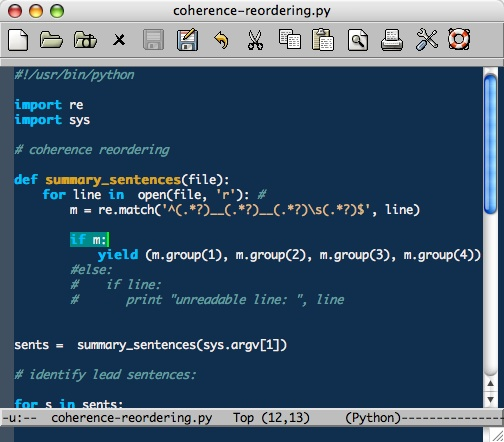
\includegraphics[width=5in]{theme.jpg}}
\caption{Aquamacs with a custom theme applied.}
\label{theme.jpg}
\end{figure}





\subsection{Buffers}
The Buffers menu allows you to navigate through the windows/frames
that you may have open. Note that a ``buffer'' is not synonymous with
a window or frame, in that you can split a frame and have more than
one buffer contained within. (Multiple windows/frames is a feature of
Aquamacs; standard Emacs does not support this.) In addition to
standard frames that display open files, there are a few other
important buffer types. One is the ``scratch'' buffer, which is simply
a buffer to type notes into; this can also be the starting point for a
file to save, and a buffer to type configuration commands for Aquamacs
(an advanced feature). Another is the ``Messages'' buffer, which
displays a log of output from Emacs commands and
operations. Finally, there is the ``info'' buffer, in which Aquamacs Emacs
displays built-in user help, tutorials and other documentation in
Emacs' ``info'' format.

 
From the Buffers menu, you can also open a new ``frame,'' or window, or
split the open window into two separate buffers. The keyboard
shortcuts for these commands are the traditional Emacs ones (see the menubar).



\begin{figure}
\centering
{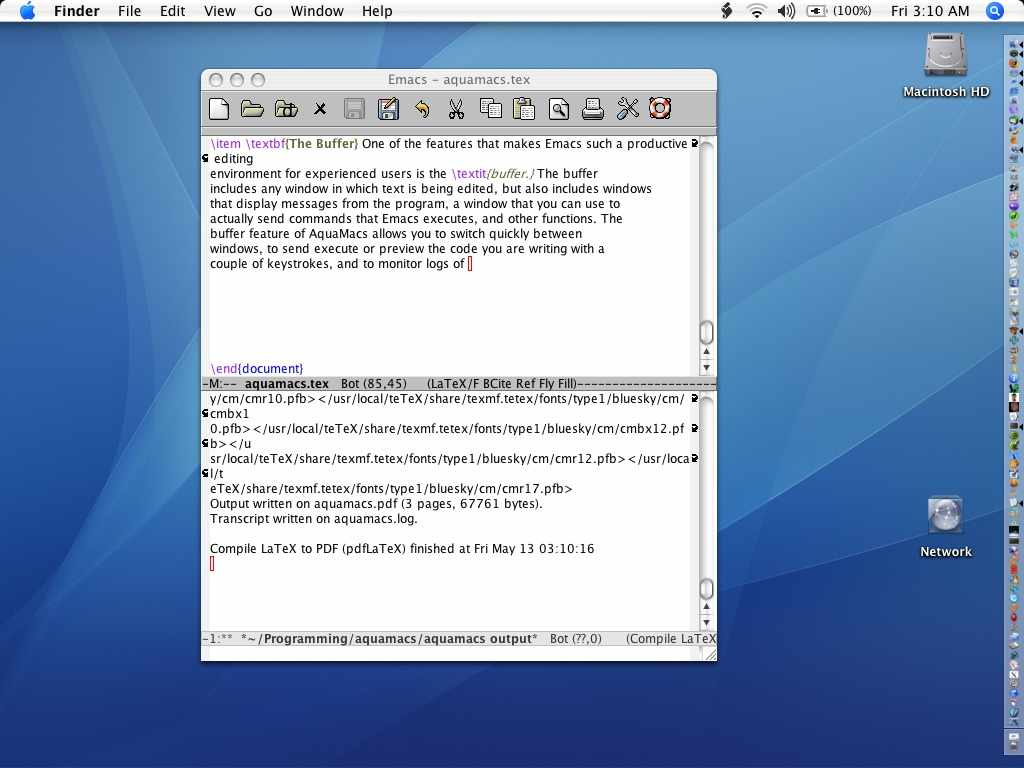
\includegraphics[width=5in]{buffers.jpg}}
\caption{The ``buffer'' feature of Emacs, which Aquamacs preserves, is
a powerful tool for enhancing productivity.}
\label{buffers.jpg}
\end{figure}

\subsection{Tools}
The Tools menu provides access to a variety of functions, including
integration with version control systems, running shell commands,
searching external files for text, and compiling and debugging
software code. The Tools menu also provides access to newsgroups and
e-mail in a command-line capacity.\footnote{The functionality
provided in the Tools menu is, to say the least, diverse, and is part
of the attraction of Emacs for a large number of users---particularly
advanced users. It is not necessary to use Aquamacs as an e-mail
client to appreciate its considerable power and utility, however.}

\subsection{Help}
The Help menu contains a wealth of information about
Aquamacs Emacs and GNU Emacs. Except for the help provided in this document,
Aquamacs' Help menu also provides documentation of the Mac-specific
customizations with the present User Manual. The general Emacs
user help is comprehensive and detailed to the point of possibly
overwhelming the inexperienced user. The beginner should definitely
start with the Emacs tutorial contained in the Help menu. While geared
toward the traditional Emacs interface instead of the OS X Aquamacs
version, the tutorial is a good introduction to Emacs' unique
capabilities. And, as you gain more experience, you will appreciate
the depth of the Emacs documentation. 

\section{Aquamacs for Emacs Veterans}

While experienced users of Emacs on other platforms can continue to
use all the key combinations to which they are accustomed, we
recommend that they use the Aquamacs-specific conventions to get the
most benefit from the applications.  Many of the
standard Emacs behaviors and interface conventions have been modified
in Aquamacs in the interest of proving a more Aqua-native
experience. In this section, we discuss some of the ways that Emacs
conventions are mapped to Aqua conventions, and outline some advanced ways that users can modify Aquamacs to their specific preferences.

\subsection{Keyboard Shortcuts}
Emacs has a well-defined set of keyboard shortcuts, which Aquamacs
revises to accomodate OS X conventions. See Table \ref{tab:shortcuts}
and Table \ref{tab:command} for details.



\begin{table}[t]
\begin{center}
 \begin{tabular}{|l|l|l|}
\hline  \textbf{Shortcut} &  \textbf{Elisp Command} &   \textbf{Function}\\ 

\hline Apple-N &new-frame-with & Create new buffer\\ &-new-scratch & \\

\hline Apple-O & mac-find-file- & Open a file\\ & other-frame & \\

\hline Apple-Shift-S & mac-save-file-as & Save as\\
 
\hline Apple-A & mark-whole-buffer & Select all text\\

\hline Apple-V & yank & Paste text\\

\hline Apple-C & clipboard-kill-ring-save & Copy text\\

\hline Apple-X &  clipboard-kill-region & Cut text\\

\hline Apple-S &  save-buffer & Save file\\

\hline Apple-L &  goto-line & Go to specified line\\

\hline Apple-F & isearch-forward & Search\\

\hline Apple-G &  isearch-repeat-forward & Repeat search\\

\hline  Apple-W &  intelligent-close & Close selected window\\

\hline Apple-M & iconify-or-deiconify- & Minimize window \\ & frame &  to the Dock\\

\hline Apple-. & keyboard-quit) & Keyboard quit\\

\hline Apple-, & customize & Show Customization Buffer\\

\hline Apple-; & toggle-mac-option- & Change Option key function\\ & modifier &\\

\hline Apple-{ / } / '& (un)comment-region-or-line & Comment out or in the \\ & current line or region if marked  &\\

\hline Apple-Backspace & kill-whole-visual-line & Deletes the current line \\
\hline Apple-Delete & kill-visual-line & Deletes the remainder of the current line \\

\hline Apple-Q & save-buffers-kill-emacs & Save file, exit program\\

\hline Apple-Z & undo & Undo\\

\hline Apple-Shift-Z &  redo & Redo\\

\hline 
\end{tabular} 
\caption{Aqua-specific keyboard shortcuts implemented in Aquamacs. }
\label{tab:shortcuts}
\end{center}
\end{table}


\begin{table}[t]
\begin{center}
 \begin{tabular}{|c|c|}
\hline \textbf{Emacs Command Key} & \textbf{Aquamacs / Mac Command Key}\\
\hline C-* & Control-*\\
\hline A-* & Apple-*\\
\hline M-* & Option-*\footnote{See setting in Options menu.}
(or Esc)\\
\hline 
\end{tabular} 
\caption{Aqua-specific command keys implemented in Aquamacs.}
\label{tab:command}
\end{center}
\end{table}


\subsection{Customizing Aquamacs}
One of the distinguishing features of Emacs is the degree to which it
can be customized by the end user. Emacs includes its own internal
scripting language, elisp, which allows the user to customize such
things as keyboard shortcuts, window settings, fonts, and more. The
Aquamacs customizations themselves are implemented in elisp.\footnote{The Aquamacs
customizations are stored in elisp files in the application bundle. It
is possible to modify these files directly, but we discourage this
practice and provide no support for it.}


We recommend that user customizations be placed in specific locations:

\begin{itemize}
\item /Library/Preferences/Emacs/Preferences.el: Preferences for all Carbon  Emacs installations
\item /Library/Preferences/Aquamacs Emacs/Preferences.el: Preferences for  Aquamacs and for all users
\item /Users/username/Library/Preferences/Emacs/Preferences.el: User-specific  preferences for all Carbon Emacs installations
\item /Users/username/Library/Preferences/Aquamacs Emacs/Preferences.el: User-specific  preferences for Aquamacs
\end{itemize}

If in doubt, use the last option:
\begin{itemize}
\item /Users/username/Library/Preferences/Aquamacs Emacs/Preferences.el
\end{itemize}

This replaces the usual ~/.emacs file, which is still loaded for  compatibility.

Below are some specific customization items that may be of interest:

\begin{itemize} 
\item \textbf{Frame.} Aquamacs opens new files (and other buffers) in
  new frames. That is usually more convenient and allows you to use
  the graphical user  interface of today's computers, which did not
  exist when Emacs was  conceived almost three decades ago. If you do
  not like this behavior, perhaps  because you are used to traditional
  Emacs, just deselect  ``Display Buffers in Separate Frames'' in the
  Options menu and save  your choice with ``Save Options.''

 
\item \textbf{mac-option-modifier.} This is  the modifier to use for the Mac alt/option key.  The value can
be alt, hyper, or super for the respective modifier.  If the value is
nil then the key will act as the normal Mac option modifier, and the option
key can be used to compose characters depending on the chosen Mac keyboard
setting. 

\item \textbf{Additional customization.} Of course, Aquamacs Emacs
  offers you almost all the customization  possibilities that Emacs
  has. Under ``Customize Emacs,'' you will find  a sub-menu that
  allows you to browse the vast space of customization
  settings. Beware: some of them are complex and not easy to
  understand. If you would like to tinker with some Aquamacs-specific
  behavior, you can customize the group ``Aquamacs.'' See Table \ref{tab:variables} for a complete list of the items that can be configured here.


\begin{table}[t]
\begin{center}
 \begin{tabular}{|l|}

\hline  \textbf{Variable}\\

\hline Aquamacs Set Creator Codes After Writing Files\\
\hline Aquamacs Quick Yes Or No Prompt\\
\hline Aquamacs Ring Bell On Error\\
\hline Aquamacs Mode Specific Default Themes\\
\hline Aquamacs Buffer Specific Frame Themes\\ 
\hline Aquamacs Auto Frame Parameters Flag\\
\hline One Buffer One Frame\\
\hline Smart Frame Positioning Enforce\\
\hline Smart Frame Positioning Mode\\
\hline Mac Option Modifier\\ 
\hline Mac Control Modifier\\ 
\hline Mac Command Modifier\\ 
\hline Aquamacs Known Buffer Modes \\
\hline
\end{tabular} 
\caption{Aquamacs-specific variables that can be customized in the Aquamacs customization group.}
\label{tab:variables}
\end{center}
\end{table}


\end{itemize}


The range of possible customizations---including restoring some of
Emacs' traditional interface conventions---is beyond the scope of this
help document. However, we provide a wiki for users to share their
modifications. See
\url{http://www.emacswiki.org/cgi-bin/wiki/AquamacsEmacs/} for more
details. 

\subsection{\LaTeX\ Support}

One special feature of Aquamacs is its extensive support for the
editing of \LaTeX documents, especially Emacs' Auc\TeX\ mode. 

\begin{figure}
\centering
{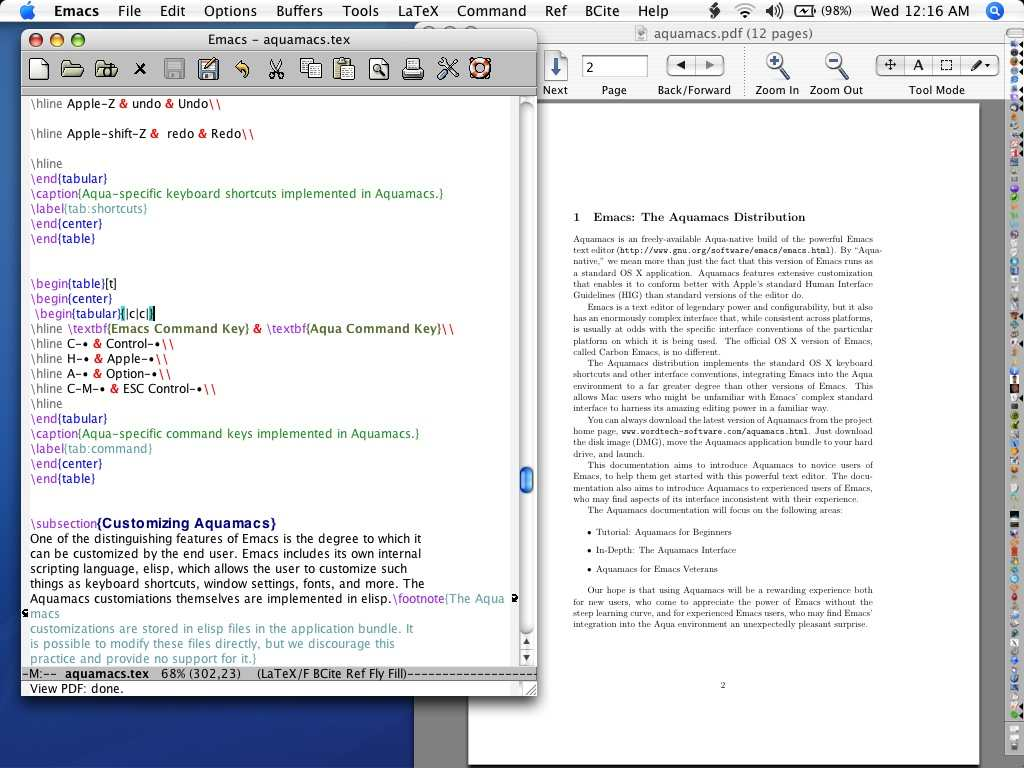
\includegraphics[width=5in]{aquamacs-tex.jpg}}
\caption{Aquamacs offers extensive support for \LaTeX\ documents.}
\label{aquamacs-tex.jpg}
\end{figure}

AUCTeX comes with its own manual, accessible via the LaTeX menu (when in latex mode after loading a .tex file), ``Read the AUCTeX manual''. If you have a question, please consult the manual. If that doesn't work, or you suspect you've found a bug in AUCTeX, please turn to the AUCTeX mailing lists, accessible here: \url{http://www.gnu.org/software/auctex/mailing-lists.html}.

To  access the enhanced \LaTeX\
functionality that Aquamacs offers, you will need to install a LaTeX system. Our recommendation:
 Install Gerben Wierda's \TeX\ package for Mac OS X. This package
  is the most complete and user-friendly \TeX\ distribution for the
  Mac. You can download the installer package at
  \url{http://www.rna.nl/tex.html}. While you can obtain \TeX\ from
  other sources,  the Gerben Wierda distribution is particularly well supported in
  Aquamacs.

\subsubsection{Enhanced Carbon Emacs Plugin Under Development}
Enrico Franconi, developer of the old Enhanced Carbon Emacs distribution that had special support for La\TeX\ editing via its customizations for Auc\TeX\ mode, has revived ECE as an external plugin that can be installed on any Carbon Emacs,including Aquamacs. At this time, the ECE plugin is undergoing beta testing. The beta version can be downloaded from this location:

\url{http://www.inf.unibz.it/~franconi/enhanced-carbon-emacs/ec-emacs-plugin-beta.dmg} 

\subsubsection{\TeX niscope: A Superb \LaTeX\ Previewer}
One special feature of the Enhanced Carbon Emacs plugin is its support
for \TeX niscope, a Cocoa-based La\TeX\ previewer that can display
both PDF and DVI formats. We recommend \TeX niscope as a superb
La\TeX\ previewer and complement to Aquamacs/Enhanced Carbon
Emacs. \TeX niscope can be downloaded from 

\noindent
\url{http://www.ing.unipi.it/~d9615/homepage/texniscope.html}.\footnote{The developer of \TeX niscope, Massimiliano Gubinelli, is also the creator of the Aquamacs icon.}

\TeX niscope needs a bit of configuration to work well with Aquamacs. See the Wiki page at \url{http://www.emacswiki.org/cgi-bin/wiki/AquamacsTexniscope} for up-to-date configuration info. 


\section{Getting Help}

There are many options for getting help with Aquamacs.

From within Aquamacs, you can access user documentation from the menu
or from specific key combinations: C-h k (key/menu entry) brings up
help for some input items; C-h f (function) gives help for an elisp
function; autocompletion support is available with (tab); and  
C-h a brings up apropos, a search function.

For help from other Aquamacs/Emacs users, the best place
to begin is the OS X Emacs mailing
list. The searchable list archives are located at
\url{http://www.esm.psu.edu/mac-tex/MacOSX-Emacs-Digests/}. For more
information on subscribing to the list, see
\url{http://aquamacs.org}.

Another option for general Emacs help is the gnu.emacs.help newsgroup.

Apart from
answering questions at the OS X Emacs mailing list, you can also file
bug reports on Aquamacs. Use the ``Send Bug Report'' function in the
Help menu  (general Emacs bugs, too), and also our Aquamacs-specific
bug report  system at \url{http://sourceforge.net/projects/aquamacs}. 

In addition to requesting help, you can also offer it in these mailing lists. \emph{Please note that in case we have helped you with a configuration problem on the mailing list, we may ask you to write a little note in the Aquamacs Wiki so others can profit, too.} Remember: Aquamacs is an Open Source community project!

\section{Donations}

Aquamacs Emacs is a project that depends on your support. You can donate very small amounts by looking at ads, or small or larger amounts directly. Both is appreciated. Your contributions will be used towards maintaining the Aquamacs web site and further development.

\url{http://aquamacs.org/donations.shtml}

\section{Acknowledgments}

We would also like to acknowledge the contributions of these authors, whose source code and hints on public forums have already been integrated into the build:
Drew Adams;
Lawrence Akka;
 Emil Astrom; 
Stefan Bruda; 
Mahn-Soo Choi;
Steve Dodd;  
Hiromatsu T.; 
Massimiliano Gubinelli (Emacs icon); 
 Kyle E. Jones; 
 Xavier Maillard;
 Pekka Marjola;
Yamamoto Mitsuharu;
Gerd Neugebauer;
 Ovidiu Predesc; 
 Alex Schr�der;
 Mikael Sj�din;
Steven Tamm; 
 Bob Weiner;  
Milan Zamazal; and 
Seiji Zenitani.

Emacs is the work of Richard Stallman and many other developers, in particular Andrew Choi (main GNU Emacs-to-MacOS/OSX port). We also would like to acknowledge the work of the authors of the major modes included.

Aquamacs Emacs is developed by David Reitter. Documentation and user support contributed by Kevin Walzer. 

Last but not least, Aquamacs couldn't exist without the dedication of its users, who donate money, report bugs and help us fix them.

\section {Licenses}

Aquamacs: the Emacs distribution, (c) 2005 by David Reitter, Kevin
Walzer and individual contributors. Aquamacs is licensed under the terms of the GNU General Public License. For details of this license, please see \url{http://www.gnu.org/copyleft/gpl.html}. The Aquamacs documentation is licensed under the terms of the GNU Free Documentation License. For details of this license, please see \url{http://www.gnu.org/copyleft/fdl.html#SEC1}.
\end{document}